\documentclass[UTF8]{ctexart}
\usepackage{titlesec}
\usepackage{fancyhdr}
\usepackage{geometry}
\usepackage{diagbox}
\usepackage{amsmath}
\usepackage{lmodern}
\usepackage{graphicx}
\usepackage{caption,subcaption}
\usepackage{wrapfig} 
\usepackage{lineno}
\geometry{left=1.0in,right=1.0in,top=0.5in,bottom=1.0in}
\pagestyle{plain}
\begin{document}

\title{\vspace{0cm}利用MLP及CNN实现图像分类}
\author{程远2234412848}
\date{}
\maketitle
\tableofcontents
\newpage
\section{引入}
计算机视觉(Computer Vesion,下面简称为CV)是一个重要的计算机科学研究领域,也是我十分感兴趣的领域。CV在如今的自动驾驶,流水线分类等方面发挥着关键性作用。
CV最基本的任务便是图像分类,该任务要求运用合适的算法,对输入图像进行分类。例如输入手写数字图像,将其分类为0-9的阿拉伯数字;
又或者输入不同的动物图片,通过计算机来分辨动物种类。最初的CV往往采用逻辑学的符号主义手段,即通过特定的识别算法,依靠各个像素点之间的差异
来识别不同的对象。然而世间万物的特征无穷无尽,识别算法却十分有限,因此CV研究陷入了停滞。然而,随着芯片算力大幅提高,神经科学中的连接主义方法
的可行性逐渐提高。程序员只需设定简单的学习模式,即可让机器从数据中自主学习出人工神经网络,从而完成图像处理任务。不难看出,神经网络在CV中起到了
革命性的影响,因此自己尝试利用神经网络完成简单的CV任务能够帮助我们对CV研究与应用的过程产生更深刻的了解,并为之后的科研工作打下基础。
\section{MLP简介}
MLP(Multilayer Perceptron,中文名多层感知机)是一种神经网络模型,本质上可以理解为一个从输入层映射到输出层的函数。
具体来说,它由一个输入层、一个或多个隐藏层和一个输出层组成。每一层中的每个神经元与下一层中的每个神经元完全连接,这种连接被称为全连接层。
除了层,激活函数也是MLP的一个重要组件,用于在模型中引入非线性。由于层与层之间都是通过线性的矩阵运算连接,因此如果不人为破坏线性,最终的输出层
一定是输入层的线性组合,这对拟合五花八门的特征显然是毁灭性的打击。所以我们们通过激活函数破坏线性,常见的激活函数有Sigmoid函数,ReLU函数等,此处不展开。

\begin{figure}[h]
    \centering
    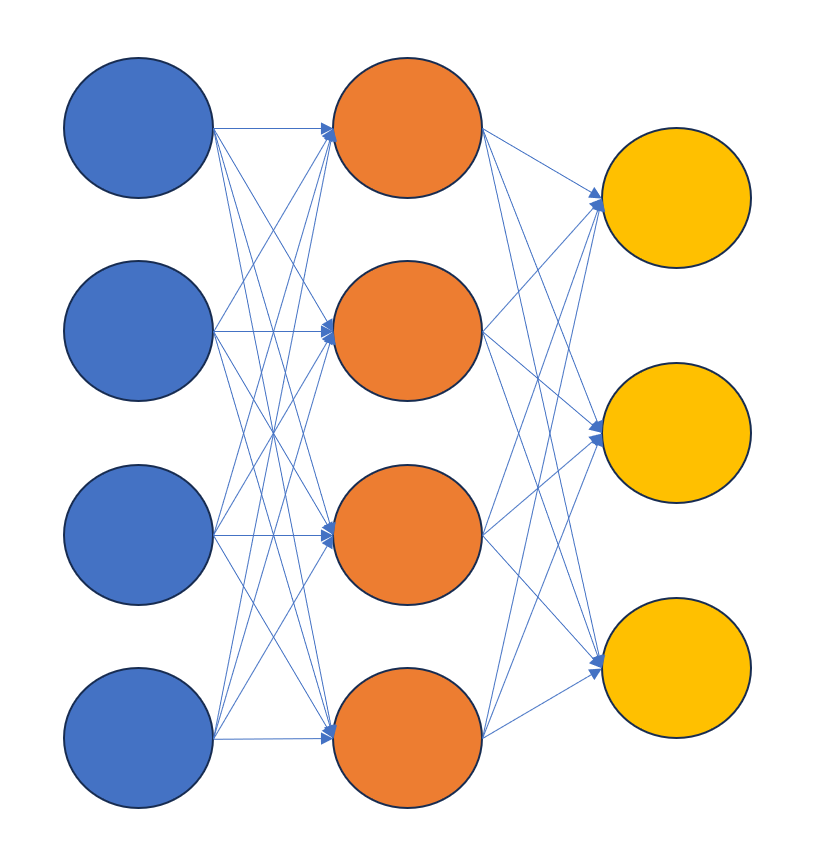
\includegraphics[width=0.5\textwidth]{MLP.png}
    \caption*{MLP结构图}
\end{figure}


\section{CNN简介}
CNN(Convolutional Neural Network,中文名CNN)也是一种神经网络模型,与MLP不同的是,CNN特别擅长处理具有网格状拓扑结构的数据,如图像和视频。
CNN通过卷积层、池化层和全连接层来提取和处理数据中的特征。它在CV任务(如图像分类、目标检测和图像分割)中表现出色。
CNN核心组件是卷积核,卷积核是一个矩阵,每一层上滑动,对应位置的数字相乘得到输出。每个卷积核产生一个特征图,多个卷积核可以提取不同的特征。
为了减少计算量和参数数量,可以通过池化层来粗略提取信息。在神经网络的最后几层,通常会添加若干层全连接层,即把CNN与MLP结合起来以提高训练效果。
\begin{figure}[h]
    \centering
    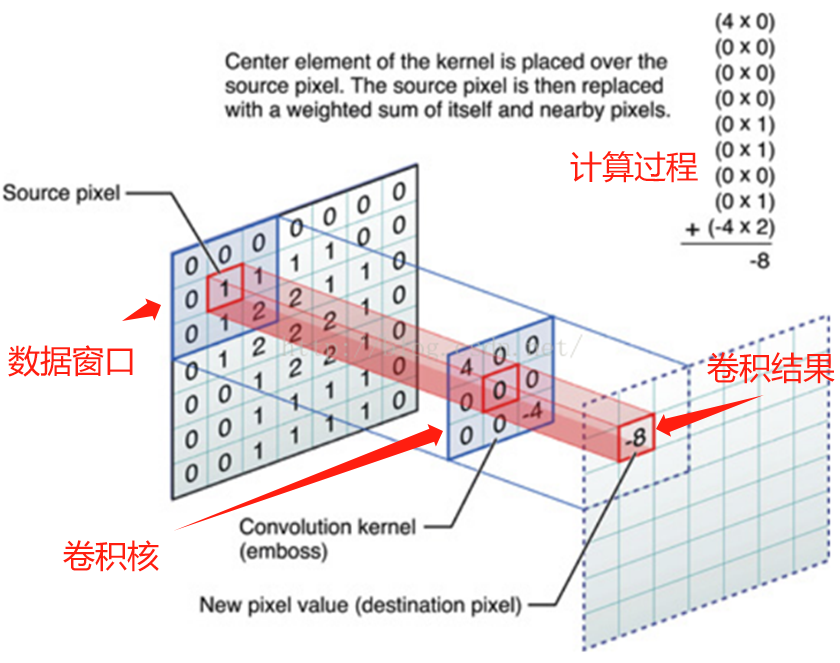
\includegraphics[width=0.8\textwidth]{CNN.png}
    \caption*{CNN计算过程演示}
\end{figure}


\section{MLP与CNN模型搭建}

\subsection{环境简介}
Windows 11 WSL2 Ubuntu 20.04 下的Pytorch,锐龙R7-5800H,RTX3050laptop。如果老师也想尝试训练模型,可能需要先行配置好pytorch环境,
详见https://blog.csdn.net/iwanvan/article/\\details/122119595

\subsection{主函数文件编写}
主函数文件为main.py,该文件下包含了训练器Trainer类的详细定义及实现。Trainer类中依次包含如下功能:构造函数、模型选择、
设置检查点、在验证集上验证模型性能、在测试集上测试模型性能、训练函数、日志记录、绘制训练效果图。
main.py的核心函数是Trainer类中的train方法,下面对其进行详细解释。首先进入外层循环,即训练epoch轮。在每一个epoch中,
通过torch自带的dataloader方法加载训练集数据并遍历数据。每一遍遍历中,先将数据加载到计算设备上(我选择的是CPU),通过模型计算出输出,
再计算损失函数,并通过反向转播更新模型参数。同时每200个step打印一次训练信息。最后将损失转换为标量保存,并进行最终的验证与测试,写入训练日志。

\subsection{模型文件}
MLP与CNN模型位于model.py中,下面依次介绍model.py中的三个模型。

第一个模型为MLP,它是一个简单的感知机,具有两个全连接层,fc1与fc2。
再初始化连接层后,需要对连接层参数进行初始化。我选择用均值为0的高斯分布初始化参数。初始化完成后,需要定义前向传播函数。
MLP的前向传播十分简单,依次进行以下操作即可:将x展平为一维张量,通过第一个全连接层的映射,应用relu激活函数,通过第二个全连接层,返回x。

第二个模型是MLP\_D,它与MLP最大的不同是添加了dropout。dropout是一种正则化技术,可以减少过拟合。dropout会在训练过程中随机丢弃神经网络中的一部分神经元,
包括其输入和输出连接。因此在每次训练迭代中,每个神经元都有一定的概率被临时排除在外,但是在下一次迭代中,这些神经元又有可能被包括进来。
这样一来,神经网络被迫在不同的神经元子集上学习,从而有效地防止神经网络在训练集上过拟合,并且通常可以显著提高在测试集上的表现。
得益于pytorch的完整框架支持,只需要额外添加一行语句“x = self.dropout(x)”就可以实现dropout的应用。

第三个模型是CNN,它是一个卷积神经网络,由若干层组成。CNN的初始化和前面的模型类似,不多赘述。下面用图展示CNN的各层神经元。
除了main.py和model.py,还有两个必要python文件:util.py与dataset.py,分别用于设置随机数与数据处理,较为简单,不展开。
\begin{figure}[h]
    \centering
    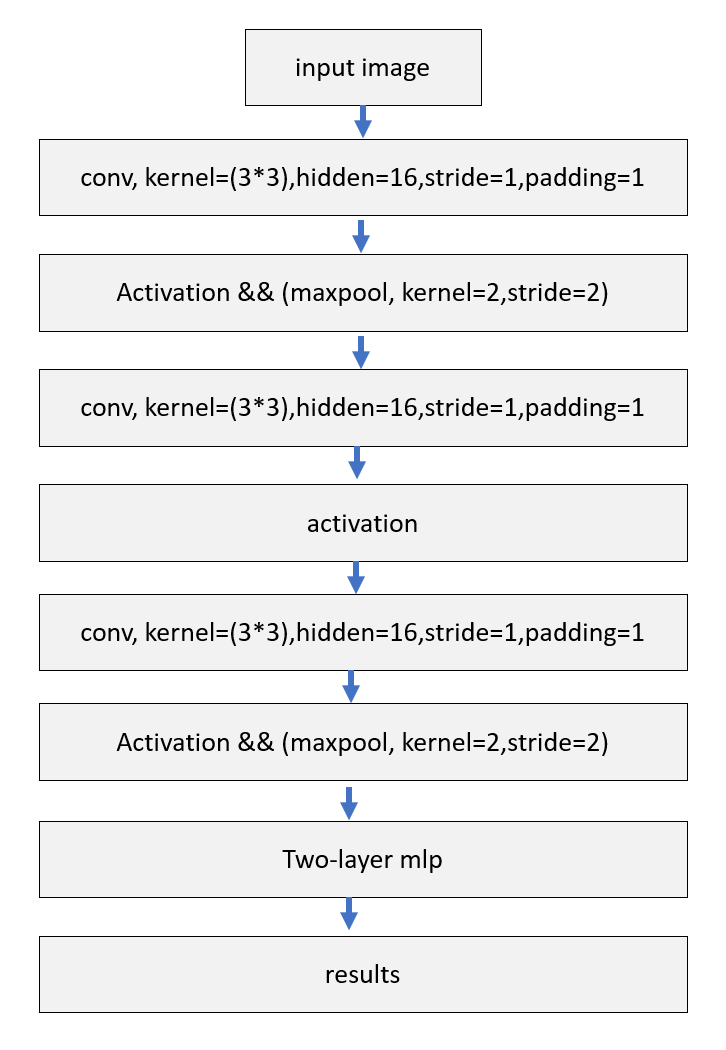
\includegraphics[width=0.4\textwidth]{CNN_MODEL.png}
    \caption*{CNN各层结构}
\end{figure}

\section{MLP与CNN模型测试}

\subsection{MLP模型测试}
在Ubuntu中输入命令python main.py,再输入MLP即可运行。前两轮运行结果如下:
\begin{figure}[h]
    \centering
    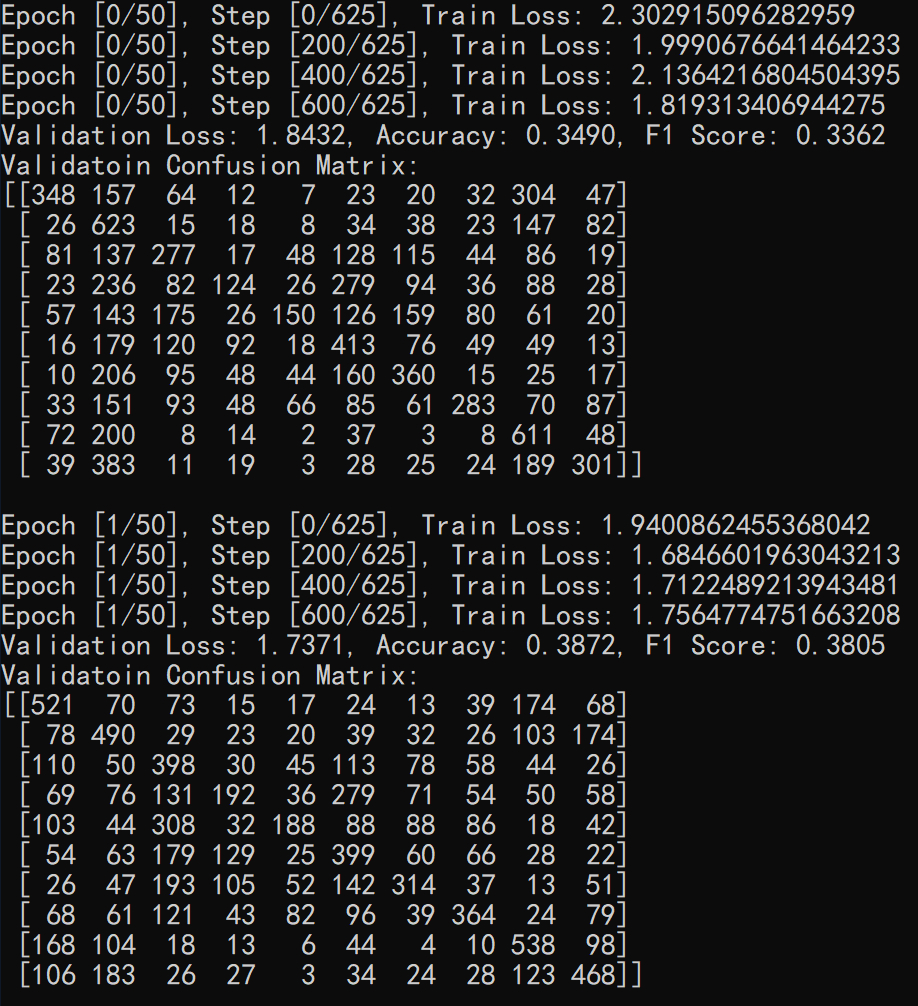
\includegraphics[width=0.8\textwidth]{MLP_run.png}
    \caption*{MLP前两轮运行结果}
\end{figure}

\newpage
训练结束后,查看日志文件,得到MLP模型最终性能如下:
\begin{figure}[h]
    \centering
    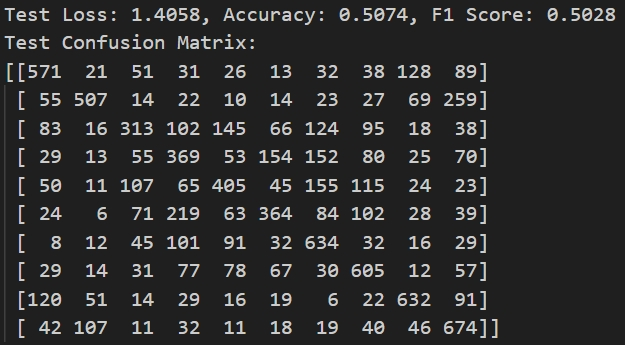
\includegraphics[width=0.8\textwidth]{MLP_res.png}
    \caption*{MLP训练结果}
\end{figure}

画出损失函数图像如下:
\begin{figure}[h]
    \centering
    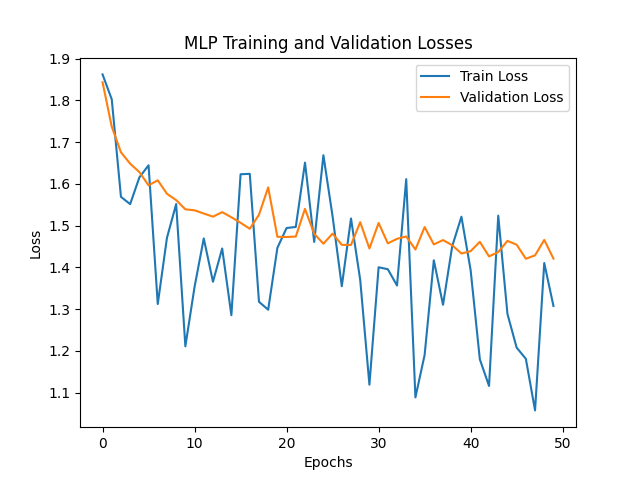
\includegraphics[width=0.7\textwidth]{MLP_loss_curve.png}
    \caption*{MLP损失函数图像}
\end{figure}

\newpage

\subsection{MLP\_D模型测试}
在Ubuntu中输入命令python main.py,再输入MLP\_D即可运行。前两轮运行结果如下:
\begin{figure}[h]
    \centering
    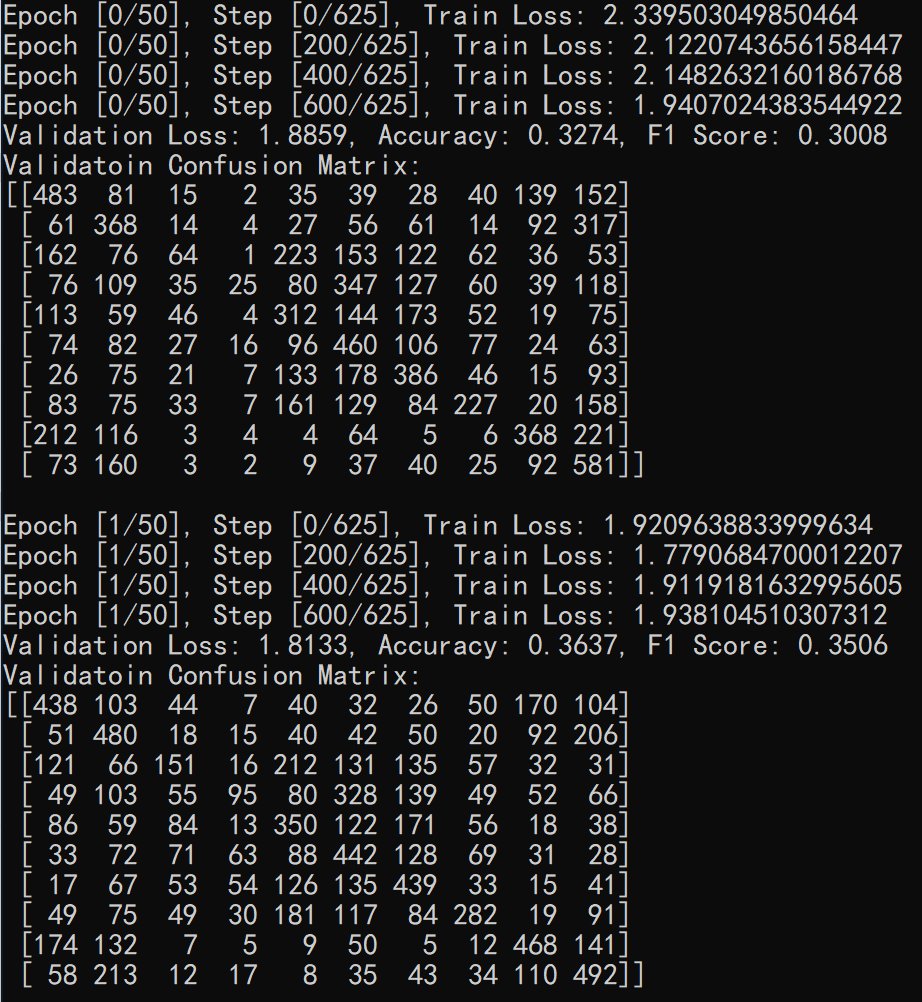
\includegraphics[width=0.8\textwidth]{MLP_D_run.png}
    \caption*{MLP\_D前两轮运行结果}
\end{figure}

\newpage

训练结束后,查看日志文件,得到MLP\_D模型最终性能如下:
\begin{figure}[h]
    \centering
    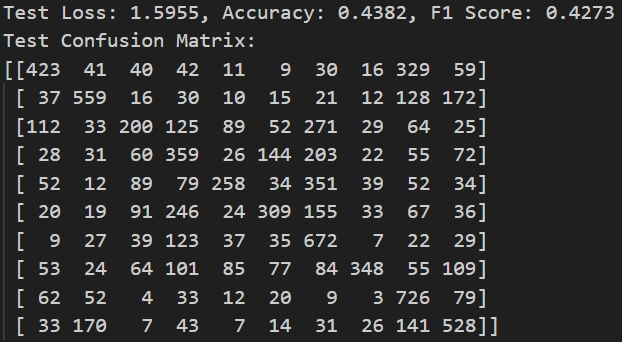
\includegraphics[width=0.8\textwidth]{MLP_D_res.png}
    \caption*{MLP\_D训练结果}
\end{figure}

画出损失函数图像如下:
\begin{figure}[h]
    \centering
    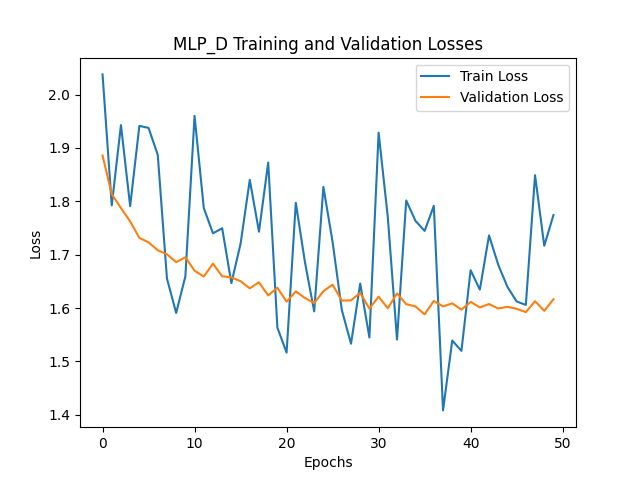
\includegraphics[width=0.7\textwidth]{MLP_D_loss_curve.png}
    \caption*{MLP\_D损失函数图像}
\end{figure}

\newpage

\subsection{CNN模型测试}
在Ubuntu中输入命令python main.py,再输入CNN即可运行。前两轮运行结果如下:
\begin{figure}[h]
    \centering
    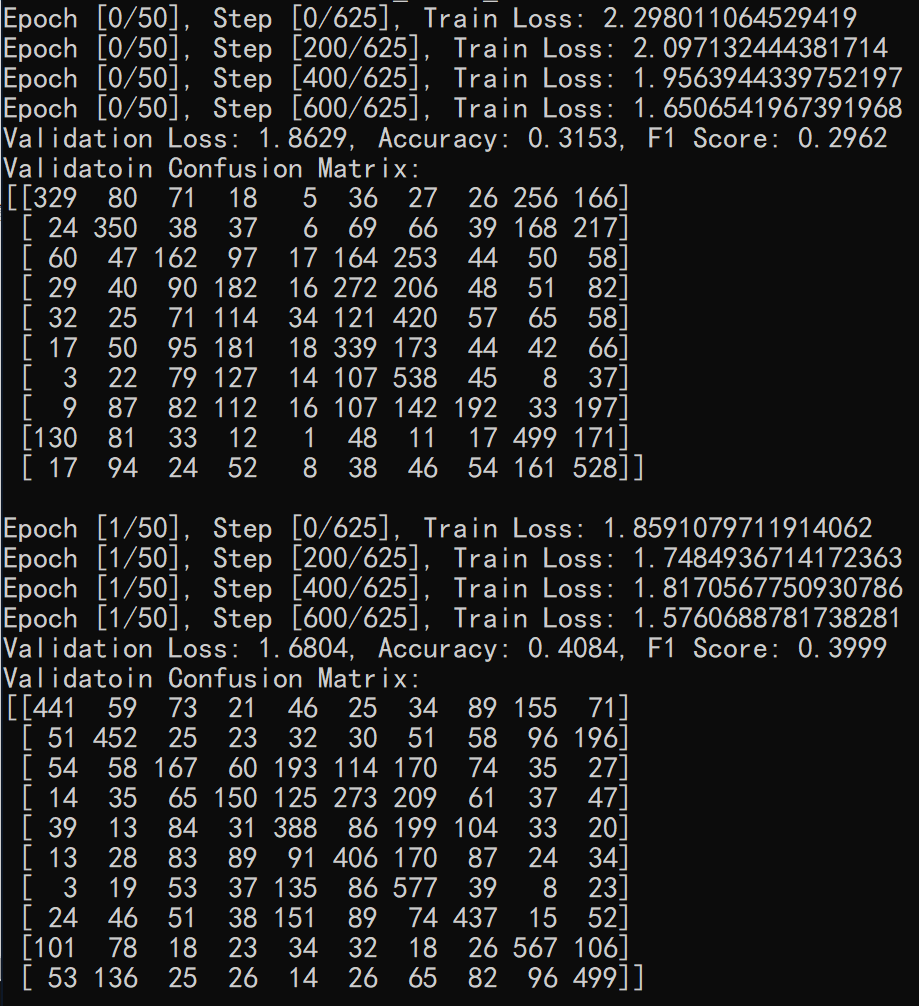
\includegraphics[width=0.8\textwidth]{CNN_run.png}
    \caption*{CNN前两轮运行结果}
\end{figure}

\newpage

训练结束后,查看日志文件,得到CNN模型最终性能如下:
\begin{figure}[h]
    \centering
    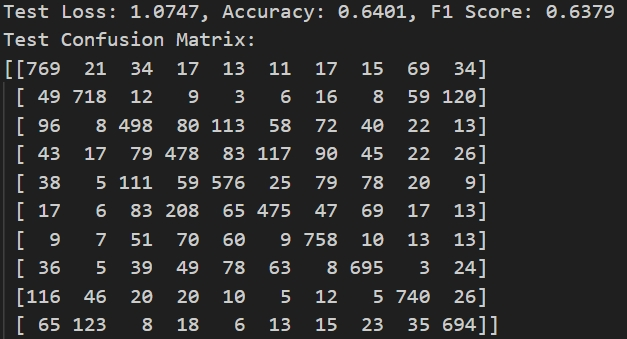
\includegraphics[width=0.8\textwidth]{CNN_res.png}
    \caption*{CNN训练结果}
\end{figure}

画出损失函数图像如下:
\begin{figure}[h]
    \centering
    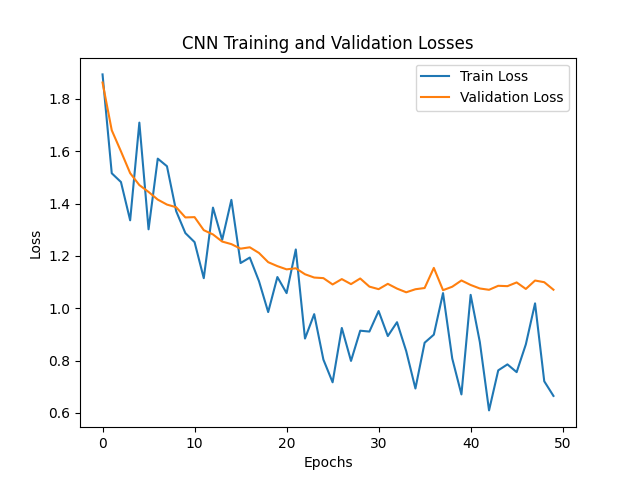
\includegraphics[width=0.7\textwidth]{CNN_loss_curve.png}
    \caption*{CNN损失函数图像}
\end{figure}

\newpage

\subsection{结果分析}
MLP是三个模型中最简单的模型,准确度最终收敛至0.5左右。然而观察其损失函数图像,发现该模型存在一定的过拟合现象。
从MLP的损失函数图像可以看出,测试集与验证集的损失数值抖动剧烈,这可能是因为模型已经毕竟拟合极限,在最优拟合左右
反复导致的。再添加dropout后,出现了两个变化。第一是测试集损失显著提高,这个容易理解。因为dropout忽略了部分神经元(我设置了忽略一半神经元),
所以模型性能有所下降,最终收敛的准确率较低。第二是验证集抖动情况得到改善,这说明模型的过拟合现象得到抑制。这两个变化
基本符合理论上的dropout作用。而CNN模型显然显示出了更强大的拟合能力,这一方面归功于卷积核能够更好地提取图像中临近像素的特征关系,
另一方面也因为我的CNN模型比MLP复杂不少,甚至CNN模型最后嵌入了两个全连接层,相当于加入了一个MLP。除了损失更低,准确率更高,CNN
的过拟合现象也更为不明显,无论是测试集损失还是验证机损失,相较MLP与MLP\_D都显得平滑不少。

\section{总结}
通过完成这次大作业,我将我对CV的兴趣转化为了现实的模型,我更好地理解了MLP和CNN的基本原理、模型结构及其在图像分类任务中的表现。
我在构建和测试MLP和CNN模型的过程中,学会了如何配置训练环境、编写训练和测试代码、以及如何分析模型的性能。
尤其是,通过对比MLP、MLP\_D(包含Dropout的MLP)和CNN模型的测试结果,我发现了不同模型在处理图像分类任务时的优缺点,以及如何通过正则化技术
(如Dropout)来减轻过拟合现象。

除了实现基本的MLP与CNN框架,我还希望未来能在更复杂的计算机视觉任务中进一步应用和优化这些模型,例如图像分割和目标检测。此外,我还计划了解并实践其他先进的神经网络结构和技术,
如生成对抗网络和注意力机制。通过不断的学习和实践,我期待能为计算机视觉领域的发展贡献自己的力量。
\section{附录:程序使用说明}
想要运行程序,主要的难点在于安装pytorch,详见https://blog.csdn.net/iwanvan/article/\\details/122119595。pytorch安装完毕后,直接将我提供的压缩包解压,
运行main.py即可。运行main.py后,程序会要求用户输入模型名称,用户需要在MLP、MLP\_D、CNN中三选一,输入后程序自动开始训练模型,训练完毕后自动测试模型并生成日志与损失函数图。

需要注意的是,用户需要基于自己的操作系统修改文件路径格式,默认为Linux路径格式。此外,用户需要在main.py的第20、21、182、184行输入想要的文件名称以及图像标题,以区分不同模型的结果。


\end{document}
